%%%%%%%%%%%%%%%%%%%%%%%%%%%%%%%%%%%%%%%%%%%%%%%%%%%%%%%%%%%%%%%%%%%%%%
%%%%  MYSTIC %%%%%%%%%%%%%%%%%%%%%%%%%%%%%%%%%%%%%%%%%%%%%%%%%%%%%%%
%%%%%%%%%%%%%%%%%%%%%%%%%%%%%%%%%%%%%%%%%%%%%%%%%%%%%%%%%%%%%%%%%%%%%%

\mysubsection{Mystic Virtues}{advancement-mystic-virtues}

\begin{center}
\myredbold{Unless otherwise specified, you can only take each Virtue once.}
\end{center}


  \mytable{Y Y Y} {
    \thead{Daredevil (Level 2+)} & \thead{Heroic (Level 4+)} & \thead{Legendary (Level 7+)} \\
  } {
    Bruja &  Cloister & Charmed Circle \\
    Charms  & Feyness & Fishers of Men \\
    Cunning Folk\Asterisk & Kismet II  & Kismet III \\
    Devotion\Asterisk & Liturgies of the Apostles &  Liturgies of the Saints  \\
    Initiate & Master of Puppets & Necromancer \\
    Kismet I  & Personality II & Norn's Shears \\
     Liturgies of the Clerics & Saves II & Personality III \\
     Medicine & Tongues of Fire & Saves III \\
     Mombo\Asterisk   & Uncanny & - \\
    Personality I  & Witch & - \\
    Sacraments &  - & - \\
     Saves I & - & - \\
     Wisdom & - & - \\
}

\callout {
    \Asterisk This Virtue can be taken once per \LVL. See details in description
}

\begin{multicols*}{2}


\myhighlight{Bruja}{adv-mystic-bruja}

Identical to the Virtue of the same name under the \mylink{Mystic Trope}{trope-mystic}.

\myhighlight{Charmed Circle}{adv-mystic-charmed-circle}

When taking \mylink{Downtime}{downtime} in a Settlement that has a \mylink{Locus}{gear-services-loci}, your brothers and sister will offer you aid and succor. They will give you information, food, and lodging for free. When figuring out how much coin you must pay for resting, treat the length of your stay as if it were one step less expensive i.e. treat Months as if you were staying for Weeks; Weeks for Days; and Days cost you nothing (staying for Years still costs the same, however). At your behest, \mylink{Mundungu}{gear-services} will summon Hekaphage to eat curses either for free or for trade (Arbiter's discretion). The amount of time to create \mylink{Marvels}{cunning-marvels} is shortened to Days; \mylink{Occultism}{cunning-marvels} that takes Months takes only Weeks, and Weeks only takes Days. Finally, the Charmed Circle grants you 4 extra Cunning Pips to use as you wish.

\myhighlight{Charms}{adv-mystic-charms}

You can perform the \mylink{Charms}{vulgate-charms} Vulgate at will.

\cbreak

\myhighlight{Cloister}{adv-mystic-cloister}

Depending on the size of the Settlement you're in, you have a chance (Small: 25\%, Medium 75\%, Large 100\%) of finding other practitioners of your faith - a coven, cult, church, or what-have-you.  Your brethren will give you information, food, and lodging for free. When figuring out how much coin you must pay for resting, treat the length of your stay as if it were one step less expensive i.e. treat Months as if you were staying for Weeks; Weeks for Days; and Days cost you nothing (staying for Years still costs the same, however). The Arbiter must share a rumor with you about your current or next adventure - the clue might be obscure, but it must be true.

\myhighlight{Cunning Folk}{adv-mystic-cunning-folk}

Identical to the Virtue of the same name under the \mylink{Mystic Trope}{trope-mystic}. If you already know this Virtue, gain 1 Cunning Pip. You can choose this Virtue once per Level.

\myimage{advancement/Mystic4}

\myhighlight{Devotion}{adv-mystic-devotion}

Gain +1 \MAX Faith, and 1 Faith Die. You can choose this Virtue once per Level.


\myhighlight{Feyness}{adv-mystic-feyness}

You can detect magic, supernatural effects, and general weirdness. 30m range for minor enchantments, charms, and sorceries; 1km range for seriously worrying magical trouble. It might be a premonition, a vision, a cold shudder, a glowing aura, or just a sense that something is "wrong". You can see ghosts and spirits, and they will know and respect you (you never need to roll \INSANITY for seeing shades or horrors). You know if an item is magical by inspecting it for Minutes.

\myhighlight{Fishers of Men}{adv-mystic-fishers-of-men}

If you take \mylink{Downtime}{downtime} in a Settlement that has a \mylink{Shrine}{gear-services-shrines} dedicated to your Small God, a member of the faithful will seek you out during the \mylink{Production Step}{downtime-production}.  If you desire, you may give this adherent one of your Faith Die to make them into a \mybold{Disciple}. The Faith die is Spent, but now resides inside of the Disciple.  Whenever you take Downtime in this Settlement, you may call upon your Disciple(s) to assist you in your \mylink{Miracle working}{wonders-miracles}. You may use the Faith die of a Disciple as if it were your own; this Faith Die can only be used once during Downtime, but will not become Spent. Should you ever suffer a \mylink{Crisis of Faith}{cruces-faith-dice-recovery}, your Disciples will immediately leave your service (even if you are not in the Settlement where they reside). You can never have more than 12 Disciples (including Vassals and Crusaders), and your Disciples will not leave the Settlement where they were first converted. They will proselytize the faith of your Small God in your absence, for good or ill.

\myhighlight{Initiate}{adv-mystic-initiate}

Identical to the Virtue of the same name under the \mylink{Mystic Trope}{trope-mystic}.

\myhighlight{Kismet I-III}{adv-mystic-kismet}

Advance \mybold{all} aspects of your \mylink{Kismet}{adventurer-kismet} to the next named level (\DEATH, \INJURY, or \INSANITY).

\myhighlight{Liturgies of the Apostles}{adv-mystic-liturgy-apostles}

If you know the Liturgy of the Clerics of a Small God, you can learn that Small God's Liturgy of the Apostles. Gain +1 \MAX Faith.

\myhighlight{Liturgies of the Clerics}{adv-mystic-liturgy-clerics}

If you know the Liturgy of the Novitiates of a Small God, you can learn that Small God's Liturgy of the Clerics. Gain +1 \MAX Faith.


\myhighlight{Liturgies of the Saints}{adv-mystic-liturgy-saints}

If you know the Liturgy of the Apostles of a Small God, you can learn that Small God's Liturgy of the Saints. Gain +1 \MAX Faith.

\newpage

\myhighlight{Master of Puppets}{adv-mystic-master-of-puppets}

During Combat, you may raise any corpses Close or Nearby as Zombie warriors. You must try your \JUJU for each warrior, but if you succeed they become "willing" combatants under your control. The Zombies will fight for as long as you maintain Concentration. Zombies always go last; you can command them at the Bottom of the Moment, and roll their attacks separately using your \FOC (in other words, treat each Zombie warrior as a \FOC weapon under your mental control). Zombies deal your \JUJU in damage if they hit (i.e. if you have d6 \JUJU, they deal d6 damage); if they themselves take any damage they collapse and are immediately consumed. Zombie warriors otherwise follow all the rules for \mylink{Zombies}{witchcraft-zombie} as defined under \mylink{Witchcraft}{arcana-witchcraft}.  At the end of Combat, all Zombie warriors will fall to the earth, and their corpses will be consumed. 

\myhighlight{Medicine}{adv-mystic-medicine}

You can perform the \mylink{Medicine}{vulgate-medicine} Vulgate during the \mylink{Shopping Step}{downtime-shopping} of \mylink{Downtime}{downtime}. 

      \myimage{advancement/LaughingMan}

\myhighlight{Mombo}{adv-mystic-mombo}

Identical to the Virtue of the same name under the \mylink{Mystic Trope}{trope-mystic}. If you already know this Virtue, gain 1 Cunning Pip. You can choose this Virtue once per Level.


\myhighlight{Necromancer}{adv-mystic-necromancer}

Advance your \mylink{Juju}{cruces-mojo-juju} \DCUP.  


\myhighlight{Norn's Shears}{adv-mystic-norns-shears}

You intercede on behalf of a member of your Band with the Fates themselves.  You can stop someone Close or Nearby from dying when there's no hope of survival, provided you can plausibly explain to the Arbiter how they survived ("she must have slipped and fallen out of the way of the dragon's breath at the last second" or "even though we saw him tumble down the Edge of the World, he must have grabbed onto a crevice").  You can only do this once, ever - and you cannot do it for yourself. 

\myhighlight{Personality I-III}{adv-mystic-personality}

Advance two \mybold{different} aspects of your \mylink{Personality}{adventurer-personality} \DCUP.


\myhighlight{Sacraments}{adv-mystic-sacraments}

You gain a single Grace die (d4) which allows you to perform the \mylink{Sacraments}{vulgate-sacraments}.

\myhighlight{Saves I-III}{adv-mystic-saves}

Advance \mybold{all} \mylink{Saves}{adventurer-saves} to the next named level (Defenseless to Preserved; Preserved to Protected; etc).

\myhighlight{Tongues of Fire}{adv-mystic-tongues-of-fire}

You can convert people to the faith of your Small God by giving them 1 of your Faith die.  The Faith die must be placed inside of a \mylink{Holy Relic}{miracle-holy-relic} and given to the initiate. Free assent is required, but it can be compelled by other factors (like a dagger to the throat or other threats). If the initiate is willing (Arbiter's discretion), gain 2 Faith.

In addition, provided you are proselytizing, you can speak (but not read) any \mylink{Dialect}{atlas-languages-dialects}.

\end{multicols*}

\newpage

\begin{center}
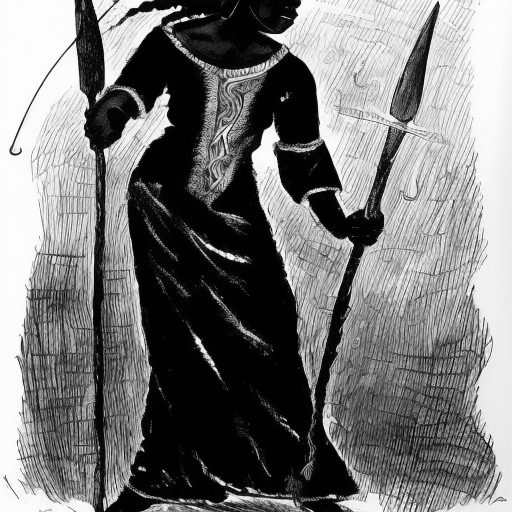
\includegraphics[scale=.6]{advancement/Mystic5}
\end{center}

\begin{multicols*}{2}


\myhighlight{Uncanny}{adv-mystic-uncanny}

Choose one of the following: 1) you take -4 damage from iron weapons (minimum 1); 2) you take -4 damage from wooden weapons (minimum 1); 3) you take -4 damage per die from non-magical fire (minimum 1 per die); 4) you are immune to drowning; 5) you take no damage from falling; 6) you take -4 damage per die from \mylink{Toxins}{malignants-toxins} (minimum 1 per die); 7) you are immune to effects of magical Charm and Sleep.


\cbreak



\myhighlight{Wisdom}{adv-mystic-wisdom}

Advance your \mylink{Juju}{cruces-mojo-juju} \DCUP.

\myhighlight{Witch}{adv-mystic-witch}

Advance your \mylink{Juju}{cruces-mojo-juju} \DCUP. 

\end{multicols*}


